% Relatorio da Fase 1 - GCC118 Programacao Matematica (UFLA, 2026/2)
% Compilar a partir desta pasta:  tectonic relatorio_fase1.tex   (ou pdflatex/xelatex)
% Numeros, tabelas e figuras sao gerados por ../analise_exploratoria.py
\documentclass[11pt,a4paper]{article}

\usepackage{iftex}
\ifPDFTeX
  \usepackage[utf8]{inputenc}
  \usepackage[T1]{fontenc}
  \usepackage{lmodern}
\else
  \usepackage{fontspec}
\fi
\usepackage[brazil]{babel}
\usepackage[margin=2.3cm]{geometry}
\usepackage{amsmath,amssymb}
\usepackage{icomma}
\usepackage{booktabs,tabularx,array}
\usepackage{graphicx}
\usepackage{float}
\usepackage[section]{placeins}
\usepackage{caption}
\usepackage{enumitem}
\usepackage[hidelinks]{hyperref}
\usepackage{xurl}

\captionsetup{font=small,labelfont=bf}
\setlist{nosep,leftmargin=*}
\graphicspath{{figuras/}}
% Gerado por fase1/analise_exploratoria.py - nao editar a mao
\newcommand{\AnoPAM}{2025}
\newcommand{\ProdBRArab}{2.230.589}
\newcommand{\ProdMGArab}{1.534.674}
\newcommand{\ProdMGCan}{29.398}
\newcommand{\PctMGBR}{68,8}
\newcommand{\ProdSul}{641.598}
\newcommand{\PctSulMG}{41,8}
\newcommand{\DifSomaMun}{0}
\newcommand{\SacasSul}{10,7}
\newcommand{\NMGCinquenta}{49}
\newcommand{\NSulCinquenta}{20}
\newcommand{\NMGOitenta}{121}
\newcommand{\NSulOitenta}{45}
\newcommand{\NMGNoventa}{165}
\newcommand{\NSulNoventa}{60}
\newcommand{\NMGNoventaCinco}{204}
\newcommand{\NSulNoventaCinco}{72}
\newcommand{\NMGCem}{462}
\newcommand{\NSulCem}{120}
\newcommand{\NMunMG}{462}
\newcommand{\NMunSul}{120}
\newcommand{\NaoDispMunMax}{47}
\newcommand{\NaoDispMunMin}{39}
\newcommand{\NaoDispSul}{2}
\newcommand{\NaoDispReg}{1.744}
\newcommand{\ZerosReg}{21.516}
\newcommand{\TotalReg}{34.080}
\newcommand{\ErroIdentMed}{0,00}
\newcommand{\ErroIdentMax}{0,1}
\newcommand{\RendMed}{1.492}
\newcommand{\RendOut}{31}
\newcommand{\CVMed}{16,7}
\newcommand{\CVPnov}{31,0}
\newcommand{\NMunCV}{120}
\newcommand{\DieselFim}{10/10/2026}
\newcommand{\DieselUlt}{7,07}
\newcommand{\DieselSemanas}{709}
\newcommand{\DieselFaltam}{10}
\newcommand{\DieselPdez}{5,91}
\newcommand{\DieselPcinq}{6,01}
\newcommand{\DieselPnov}{6,99}
\newcommand{\DieselSpread}{-2,6}
\newcommand{\PostosMed}{309}
\newcommand{\NNosOSRM}{36}
\newcommand{\NParesOSRM}{1.254}
\newcommand{\CircMed}{1,39}
\newcommand{\CircMedia}{1,42}
\newcommand{\CircPdez}{1,25}
\newcommand{\CircPnov}{1,63}
\newcommand{\VelMed}{61,1}
\newcommand{\AssimMed}{0,2}
\newcommand{\AssimMax}{23,8}
\newcommand{\SnapMax}{225}
\newcommand{\ViagensAno}{21.387}
\newcommand{\ViagensDia}{86}
\newcommand{\TonDia}{2.566}
\newcommand{\DiasUteis}{250}
\newcommand{\CapQ}{30}
\newcommand{\NOtimoNivelUm}{8}


\title{\textbf{Logística de café até portos secos}\\[2pt]
\large Fase 1: análise exploratória (tamanho da instância, qualidade e viabilidade dos dados)}
\author{Giovane Felipe Godoi Oliveira \quad Luiz Fellipe Resende Lima\\
\small GCC118 Programação Matemática, UFLA, semestre 2026/2\\
\small Docentes: Mayron César O. Moreira e Andreza C. Beezão Moreira}
\date{Outubro de 2026}

\begin{document}
\maketitle

\begin{abstract}
\noindent
Este relatório caracteriza os dados públicos que alimentam o problema de roteamento de café até portos secos
(Opção A do trabalho prático). Foram coletados a produção municipal de café da PAM/IBGE (\AnoPAM), a série semanal de
preço do diesel da ANP (até \DieselFim), a lista oficial de recintos alfandegados de Minas Gerais e uma matriz
rodoviária de distância e tempo calculada no OSRM. O Sul/Sudoeste de Minas produziu \ProdSul~t de café arábica em
\AnoPAM{} (\PctSulMG\% de MG). Cobrir 80\% dessa produção exige \NSulOitenta{} municípios, o que leva o modelo PLI do
Nível 1 a \BinOitenta{} variáveis binárias. São \RazaoBin{} vezes mais que na maior instância que o solver resolveu
com prova de otimalidade (\NOtimoNivelUm{} coletas). Os dados de localização, distância, tempo e combustível são públicos e de boa
qualidade. Estoques por propriedade, tipos comerciais de café (necessários para os \emph{blends}), silos e tarifas de
terminais não são públicos e serão tratados como parâmetros sintéticos documentados. A conclusão é que o problema é
viável com instâncias \emph{semi-reais}: geografia, distâncias e custos reais, e oferta e composição sintéticas, mas
calibradas pela PAM.
\end{abstract}

\section{Problema e objetivo desta fase}

O problema é planejar a coleta de café em pontos de oferta (municípios ou armazéns) e a entrega em portos secos,
minimizando o custo logístico total (veículos, deslocamento e entrada no terminal). No Nível 1 o modelo é um CVRP com
escolha do porto seco: frota homogênea de capacidade $Q$, um produto e um terminal por rota. A extensão em estudo
(\emph{blends}) acrescenta tipos de café armazenados em silos diferentes e uma passagem obrigatória por uma
misturadora antes do porto seco.

A Fase 1 responde a três perguntas, uma por seção:
\begin{enumerate}
  \item \textbf{Tamanho} (Seção~\ref{sec:tamanho}): quantos pontos, terminais e viagens tem a instância real, e o modelo
        exato consegue resolvê-la?
  \item \textbf{Qualidade} (Seção~\ref{sec:qualidade}): os dados públicos são completos, consistentes e adequados ao
        uso que o modelo faz deles?
  \item \textbf{Viabilidade} (Seção~\ref{sec:viabilidade}): que parâmetros podem ser obtidos de fontes públicas e quais
        precisam ser assumidos?
\end{enumerate}

\textbf{Escopo geográfico.} Minas Gerais produziu \PctMGBR\% do café arábica do Brasil em \AnoPAM{}
(Tabela~\ref{tab:producao_anual}). A análise se concentra na mesorregião Sul/Sudoeste de Minas, a maior região produtora
do estado e a mais próxima dos CLIAs de Varginha e Pouso Alegre (Figura~\ref{fig:mapa}).

\section{Fontes e coleta}\label{sec:fontes}

Toda a coleta é reproduzível pelo script \texttt{fase1/coleta\_dados.py}, que baixa as fontes brutas e grava tabelas
limpas em \texttt{dados/processados}. O script \texttt{fase1/analise\_exploratoria.py} gera todas as figuras, tabelas e
números deste relatório. A Tabela~\ref{tab:fontes} lista as fontes.

\begin{table}[htbp]
\centering\small
\caption{Fontes de dados usadas e parâmetro do modelo que cada uma alimenta.}\label{tab:fontes}
\begin{tabularx}{\linewidth}{>{\raggedright}p{3.2cm} >{\raggedright}X >{\raggedright\arraybackslash}p{4.1cm}}
\toprule
Fonte & Conteúdo extraído & Uso no modelo \\
\midrule
PAM/IBGE, SIDRA tabela 1613 & Produção (t), área colhida (ha), rendimento (kg/ha) e valor, por município, de 2021 a
\AnoPAM, café arábica e canephora & oferta $q_i$ dos pontos de coleta; escolha do escopo \\
IBGE Localidades & meso e microrregião, região intermediária & recorte regional \\
Sedes municipais (base aberta \url{kelvins/municipios-brasileiros}) & latitude e longitude & coordenadas dos nós \\
ANP, levantamento semanal por estado & preço médio, mínimo e máximo do diesel S10 e S500 em MG, 2013 a \DieselFim
& preço $p$ do diesel e cenários \\
Receita Federal, lista de portos secos (fev/2023) & recintos de Juiz de Fora e Uberaba & conjunto $D$ de terminais \\
Ata da 2ª reunião Colfac-MG (nov/2022) & CLIAs de Varginha, Pouso Alegre e Betim & conjunto $D$ de terminais \\
OSRM (OpenStreetMap) & matriz \NNosOSRM$\times$\NNosOSRM{} de distância e tempo rodoviário & $\delta_{ij}$, $t_{ij}$ e
$c_{ij}$ \\
\bottomrule
\end{tabularx}
\end{table}

\textbf{Definição de terminal.} A Receita Federal separa os portos secos dos Centros Logísticos e Industriais
Aduaneiros (CLIA). Na lista oficial, Minas Gerais tem dois portos secos em sentido estrito: Juiz de Fora (Multiterminais,
recinto 6.35.32.01-8) e Uberaba (Porto Seco do Triângulo, 6.45.32.01-1). Os três CLIAs (Varginha, Pouso Alegre e Betim)
cumprem a mesma função logística de recinto alfandegado de zona secundária. Neste trabalho, ``porto seco'' é usado no
sentido operacional e inclui os cinco recintos ($m = 5$).

\section{Análise exploratória}\label{sec:eda}

\subsection{Produção de café}

\begin{table}[htbp]
\centering
\small
\caption{Produção de café em grão (PAM/IBGE, tabela 1613).}
\label{tab:producao_anual}
\begin{tabular}{lrrrrr}
\toprule
Ano & Brasil arábica (t) & MG arábica (t) & Sul/Sudoeste MG (t) & Var. Sul (\%) & MG canephora (t) \\
\midrule
2021 & 1.979.430 & 1.343.980 & 566.911 & -- & 15.848 \\
2022 & 2.071.598 & 1.373.871 & 521.753 & -8,0 & 23.399 \\
2023 & 2.364.611 & 1.714.053 & 669.058 & 28,2 & 21.355 \\
2024 & 2.393.487 & 1.663.992 & 706.554 & 5,6 & 23.337 \\
2025 & 2.230.589 & 1.534.674 & 641.598 & -9,2 & 29.398 \\
\bottomrule
\end{tabular}
\par\smallskip\footnotesize\raggedright Fonte: SIDRA/IBGE, extraído pelo script \texttt{coleta\_dados.py}. A soma municipal de MG coincide com o total estadual publicado.
\end{table}


A Tabela~\ref{tab:producao_anual} e a Figura~\ref{fig:serie} mostram a série de 2021 a \AnoPAM. A produção varia de
forma relevante de um ano para outro, como esperado pela \emph{bienalidade} do arábica (alternância entre safras
altas e baixas). Por isso a oferta $q_i$ não deve ser tratada como um número fixo: na Fase 4 ela entra como fonte de
incerteza. No Sul/Sudoeste, o coeficiente de variação municipal da produção nos cinco anos tem mediana de \CVMed\% e
percentil 90 de \CVPnov\% (\NMunCV{} municípios com produção em todos os anos).

\begin{figure}[htbp]
\centering
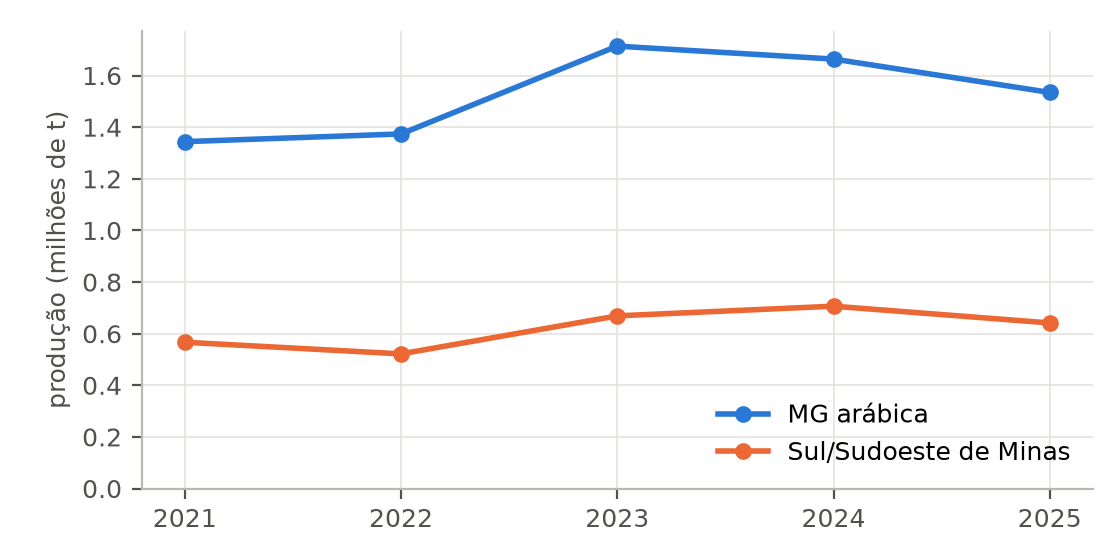
\includegraphics[width=0.75\linewidth]{serie_anual.png}
\caption{Produção anual de café arábica em MG e no Sul/Sudoeste de Minas (PAM/IBGE).}\label{fig:serie}
\end{figure}

\begin{figure}[htbp]
\centering
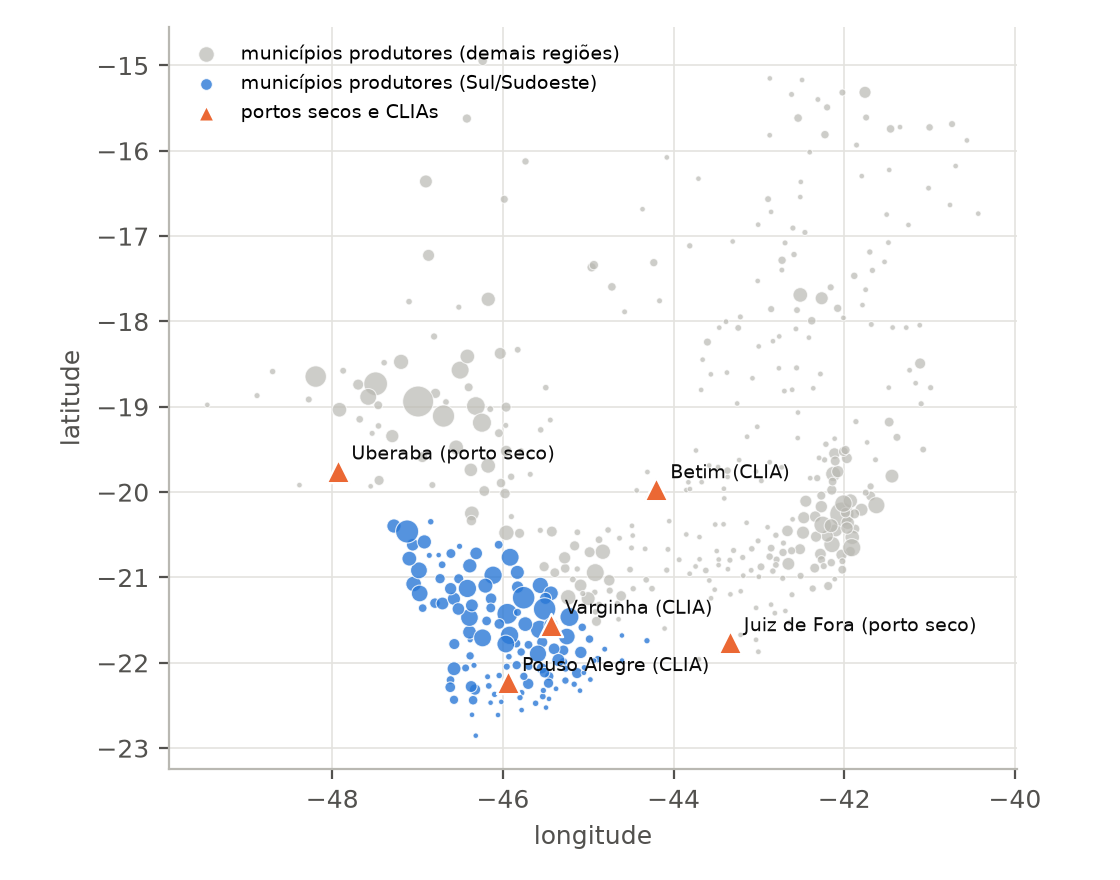
\includegraphics[width=0.78\linewidth]{mapa.png}
\caption{Municípios produtores de café arábica em \AnoPAM{} (área do círculo proporcional à produção) e recintos
alfandegados de MG. Coordenadas das sedes municipais.}\label{fig:mapa}
\end{figure}

A produção é concentrada (Figura~\ref{fig:concentracao} e Tabela~\ref{tab:concentracao}). Em MG, \NMunMG{} municípios
produziram arábica em \AnoPAM, mas \NMGOitenta{} deles respondem por 80\% do total. No Sul/Sudoeste, \NSulCinquenta{}
municípios cobrem metade da produção e \NSulOitenta{} cobrem 80\%. Essa concentração define os tamanhos de instância
da Seção~\ref{sec:tamanho}. A Figura~\ref{fig:top} mostra os maiores produtores da região, que também são os pontos de
coleta da matriz OSRM.

\begin{figure}[htbp]
\centering
\begin{minipage}{0.52\linewidth}\centering
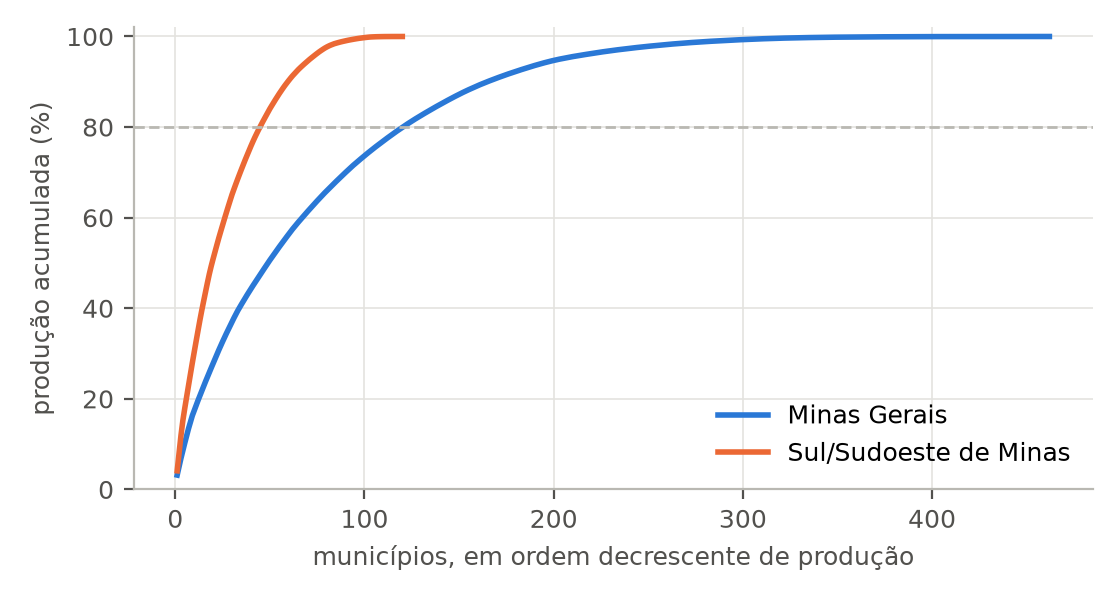
\includegraphics[width=\linewidth]{concentracao.png}
\caption{Curva de concentração da produção de arábica (\AnoPAM).}\label{fig:concentracao}
\end{minipage}\hfill
\begin{minipage}{0.45\linewidth}\centering
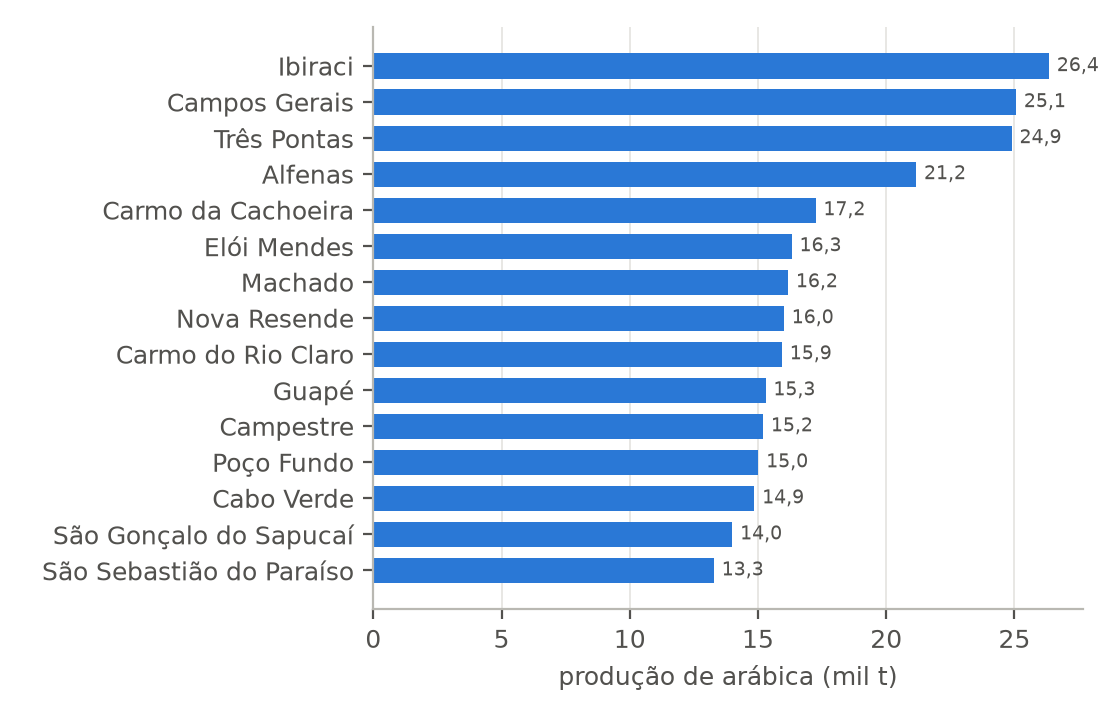
\includegraphics[width=\linewidth]{top_sul.png}
\caption{Os 15 maiores produtores do Sul/Sudoeste de Minas (\AnoPAM).}\label{fig:top}
\end{minipage}
\end{figure}

\begin{table}[htbp]
\centering
\small
\caption{Número de municípios necessários para cobrir uma fração da produção de arábica (2025).}
\label{tab:concentracao}
\begin{tabular}{lrr}
\toprule
Fração da produção & Municípios MG & Municípios Sul/Sudoeste \\
\midrule
50\% & 49 & 20 \\
80\% & 121 & 45 \\
90\% & 165 & 60 \\
95\% & 204 & 72 \\
100\% & 462 & 120 \\
\bottomrule
\end{tabular}
\end{table}


\subsection{Terminais e distâncias}

A matriz OSRM tem \NNosOSRM{} nós: a garagem (Varginha, base assumida da frota), os 30 maiores produtores do
Sul/Sudoeste e os cinco recintos. A Tabela~\ref{tab:dist_terminais} mostra que os CLIAs de Varginha e Pouso Alegre ficam
dentro da região produtora, enquanto Juiz de Fora, Uberaba e Betim estão a 4--7 horas de viagem. É exatamente esse
contraste que torna interessante a escolha do terminal: um terminal distante só compensa se tiver custo de entrada ou
tarifa menor, ou se ficar mais perto do porto marítimo de destino.

\begin{table}[htbp]
\centering
\small
\caption{Distância rodoviária (OSRM) dos 30 maiores municípios produtores do Sul/Sudoeste até cada recinto alfandegado.}
\label{tab:dist_terminais}
\begin{tabular}{lrrr}
\toprule
Terminal & Dist. média (km) & Dist. mín.--máx. (km) & Tempo médio (h) \\
\midrule
Juiz de Fora (porto seco) & 413 & 280--623 & 6,7 \\
Uberaba (porto seco) & 333 & 124--473 & 4,7 \\
Varginha (CLIA) & 128 & 0--318 & 2,1 \\
Pouso Alegre (CLIA) & 177 & 60--377 & 2,8 \\
Betim (CLIA) & 331 & 229--453 & 4,7 \\
\bottomrule
\end{tabular}
\end{table}


A Figura~\ref{fig:circuidade} compara a distância rodoviária com a distância em linha reta em \NParesOSRM{} pares de
nós. O \emph{fator de circuidade} (rodoviária/linha reta) tem mediana \CircMed{} (P10 = \CircPdez, P90 = \CircPnov). Esse
valor é \textbf{maior} que o fator 1,25 usado nas instâncias sintéticas do Nível 1, que portanto subestimavam as
distâncias em cerca de 10\%. A velocidade média implícita no OSRM é de \VelMed{} km/h, o que confirma a hipótese de
60 km/h. A matriz é quase simétrica: a assimetria relativa tem mediana de \AssimMed\% e máximo de \AssimMax\%. Mesmo
assim, ela será tratada como direcionada, como recomenda a modelagem.

\begin{figure}[htbp]
\centering
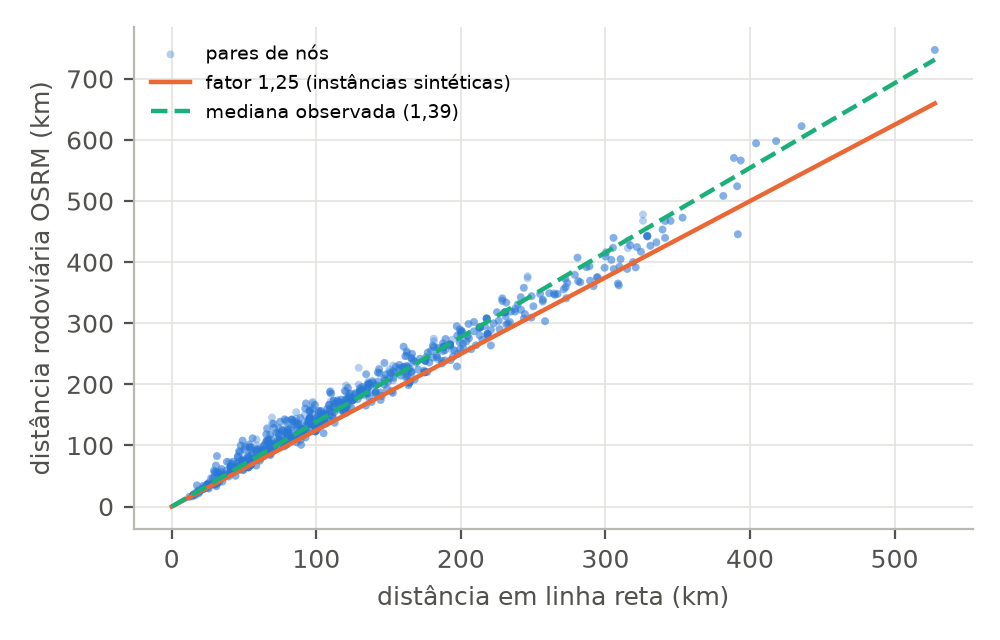
\includegraphics[width=0.66\linewidth]{circuidade.png}
\caption{Distância rodoviária (OSRM) versus distância em linha reta entre os nós da instância.}\label{fig:circuidade}
\end{figure}

\subsection{Preço do diesel}

A série semanal da ANP para MG tem \DieselSemanas{} semanas de diesel S10, de 2013 a \DieselFim{}
(Figura~\ref{fig:diesel}). O preço nominal triplicou no período e teve choques em 2022 e 2026. Nas últimas 104 semanas,
a mediana foi de R\$~\DieselPcinq/L. O último preço observado (R\$~\DieselUlt/L) está acima do percentil 90 da
janela, o que reforça a necessidade de analisar cenários. A Tabela~\ref{tab:diesel} traduz os percentis em custo por
quilômetro. No cenário base, o diesel responde por \PctDieselKm\% do custo variável por km, e o custo por km do cenário alto
é \CustoKmDif\% maior que o do cenário baixo.

\begin{figure}[htbp]
\centering
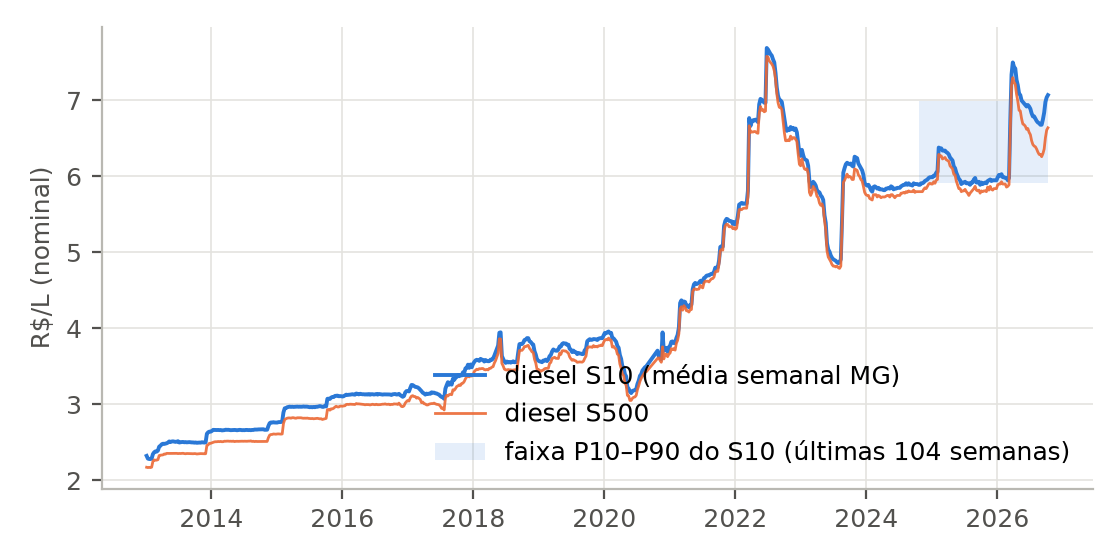
\includegraphics[width=0.78\linewidth]{diesel.png}
\caption{Preço médio semanal de revenda do diesel em MG (ANP), em valores nominais.}\label{fig:diesel}
\end{figure}

\begin{table}[htbp]
\centering
\small
\caption{Cenários de preço do diesel S10 em MG (últimas 104 semanas) e custo por quilômetro.}
\label{tab:diesel}
\begin{tabular}{lrr}
\toprule
Cenário & Diesel S10 (R\$/L) & Custo por km (R\$/km) \\
\midrule
baixo (P10) & 5,91 & 5,16 \\
base (P50) & 6,01 & 5,20 \\
alto (P90) & 6,99 & 5,60 \\
\bottomrule
\end{tabular}
\par\smallskip\footnotesize\raggedright Custo por km $= c^{km} + p\,g$, com $c^{km} = 2,80$ R\$/km e $g = 0,40$ L/km (hipóteses do Nível 1).
\end{table}


\section{Qualidade dos dados}\label{sec:qualidade}

A Tabela~\ref{tab:qualidade} resume as verificações feitas e o tratamento adotado.

\begin{table}[htbp]
\centering\small
\caption{Verificações de qualidade e tratamento adotado.}\label{tab:qualidade}
\begin{tabularx}{\linewidth}{>{\raggedright}p{3.0cm} >{\raggedright}X >{\raggedright\arraybackslash}p{4.4cm}}
\toprule
Item & Constatação & Tratamento \\
\midrule
Completude da PAM & De \TotalReg{} registros (município $\times$ variável $\times$ ano $\times$ espécie), \ZerosReg{}
têm o código ``-'' (zero absoluto) e \NaoDispReg{} têm ``...'' (não disponível). Os ``...'' cobrem de \NaoDispMunMin{} a
\NaoDispMunMax{} municípios por ano, sem registro de lavoura, e só \NaoDispSul{} deles ficam no Sul/Sudoeste em
\AnoPAM. & ``-'' vira 0. ``...'' fica ausente e o município é excluído do escopo, sem imputação. \\
Consistência interna & A soma municipal de MG difere do total estadual publicado em \DifSomaMun~t. A identidade
produção = área $\times$ rendimento tem erro mediano de \ErroIdentMed\% e máximo de \ErroIdentMax\% (arredondamento). &
Dados consistentes; nenhuma correção. \\
Valores atípicos & Rendimento mediano de \RendMed~kg/ha (faixa de \RendMin{} a \RendMax~kg/ha). \RendOut{} municípios
ficam fora de 1,5 IQR, sem indício de erro de registro, porque a identidade com área e produção se mantém. & Mantidos;
não afetam $q_i$, que usa a produção. \\
Natureza da PAM & É uma estimativa anual da produção do município, não o estoque disponível nem o volume exportado. &
$q_i$ é derivado da produção por uma regra explícita (Seção~\ref{sec:tamanho}). \\
Variabilidade & Bienalidade: CV municipal mediano de \CVMed\% em cinco anos. & Cenários de oferta na Fase 4. \\
Série ANP & \DieselFaltam{} semanas sem pesquisa (ago/2015 e ago--out/2020). Houve mudanças de metodologia e de
amostra (cerca de \PostosMed{} postos por semana em MG). & Uso só das últimas 104 semanas, sem lacunas; valores nominais. \\
Coordenadas & As sedes municipais representam os pontos de coleta e os terminais. O OSRM deslocou os pontos até a
via mais próxima em no máximo \SnapMax~m. & Aceitável para instâncias agregadas. Portões dos recintos a
georreferenciar. \\
Matriz OSRM & Servidor público de demonstração, perfil de automóvel e sem restrições de caminhão nem pedágio. &
Tempos são limite inferior; pedágio (ANTT) fica como extensão. \\
\bottomrule
\end{tabularx}
\end{table}

\section{Tamanho da instância}\label{sec:tamanho}

\textbf{Volume físico.} O Sul/Sudoeste produziu \ProdSul~t em \AnoPAM{} (cerca de \SacasSul{} milhões de sacas de
60 kg). Com caminhões de $Q = \CapQ$~t, isso equivale a \ViagensAno{} viagens por ano. Supondo \DiasUteis{} dias de
expedição, são cerca de \TonDia~t e \ViagensDia{} viagens por dia, se toda a produção passasse pelos recintos. Esse
número é um limite superior, porque parte do café vai para torrefação interna ou é exportada por outros canais. Mesmo
assim, a escala real é de dezenas de rotas por dia e não de uma ou duas.

\textbf{Tamanho do modelo.} O modelo do Nível 1 tem $n + n(n-1) + nm$ variáveis binárias. A Tabela~\ref{tab:tamanho}
aplica essa fórmula aos escopos definidos pela concentração da produção. A Tabela~\ref{tab:escalabilidade} mostra o
comportamento observado do solver: com o limite de 20 s, o CBC prova o ótimo até $n = \NOtimoNivelUm$ coletas, e
com $n = 9$ já atinge o limite.

\begin{table}[htbp]
\centering
\small
\caption{Tamanho do modelo PLI do Nível 1 em função do escopo da instância real.}
\label{tab:tamanho}
\begin{tabular}{lrrrrr}
\toprule
Escopo & $n$ & $m$ & Binárias & Contínuas & Restrições (aprox.) \\
\midrule
instância de teste (Nível 1) & 8 & 5 & 104 & 16 & 174 \\
50\% da produção do Sul/Sudoeste & 20 & 5 & 500 & 40 & 906 \\
80\% da produção & 45 & 5 & 2.250 & 90 & 4.281 \\
90\% da produção & 60 & 5 & 3.900 & 120 & 7.506 \\
todos os produtores & 120 & 5 & 15.000 & 240 & 29.406 \\
\bottomrule
\end{tabular}
\par\smallskip\footnotesize\raggedright Binárias $= n + n(n-1) + nm$; restrições $\approx 2n + m + 1 + 2n(n-1) + nm$ (fluxo, carga, tempo e terminal), conforme \texttt{02\_modelo\_PLI\_nivel1.md}.
\end{table}

\begin{table}[htbp]
\centering
\small
\caption{Escalabilidade do modelo exato do Nível 1 (CBC, limite de 20 s, instâncias sintéticas).}
\label{tab:escalabilidade}
\begin{tabular}{rrrrrc}
\toprule
$n$ & Binárias & Variáveis & Restrições & Tempo (s) & Ótimo provado \\
\midrule
4 & 24 & 34 & 76 & 0,05 & sim \\
5 & 35 & 47 & 109 & 0,12 & sim \\
6 & 48 & 62 & 148 & 0,19 & sim \\
7 & 63 & 79 & 193 & 1,72 & sim \\
8 & 80 & 98 & 244 & 5,74 & sim \\
9 & 99 & 119 & 301 & 20,01 & não \\
10 & 120 & 142 & 364 & 20,01 & não \\
\bottomrule
\end{tabular}
\end{table}


\textbf{Conclusão sobre o tamanho.} Uma instância que cubra 80\% da produção regional ($n = \NSulOitenta$, \BinOitenta{}
binárias) tem \RazaoBin{} vezes mais binárias que a maior instância resolvida com prova de otimalidade, e o número
de rotas possíveis cresce de forma fatorial com $n$. Pelo
enunciado, isso pede uma adaptação justificada. Ela será tratada nas Fases 2 e 3:
\begin{enumerate}
  \item \textbf{Restrição de escopo:} instâncias diárias com os $n$ municípios de maior oferta no dia (de 8 a 20 pontos),
        que é o horizonte real de planejamento de uma cooperativa.
  \item \textbf{Decomposição:} agrupar os municípios por terminal mais próximo e resolver cada grupo separadamente,
        usando a política ``porto mais próximo'' do Nível 1 como limite superior.
  \item \textbf{Heurística:} construção mais busca local na instância completa, comparada ao exato onde ele ainda prova
        otimalidade.
\end{enumerate}

\section{Viabilidade dos dados}\label{sec:viabilidade}

A Tabela~\ref{tab:viabilidade} classifica cada parâmetro do modelo, incluindo a extensão dos \emph{blends}.

\begin{table}[htbp]
\centering\small
\caption{Disponibilidade dos parâmetros do modelo.}\label{tab:viabilidade}
\begin{tabularx}{\linewidth}{>{\raggedright}p{4.0cm} >{\raggedright}p{2.6cm} >{\raggedright\arraybackslash}X}
\toprule
Parâmetro & Situação & Observação \\
\midrule
Localização dos pontos de coleta & público & sedes municipais (IBGE); fazendas exigiriam CAR/SICAR e o ponto de acesso \\
Oferta $q_i$ & derivado & proporcional à produção PAM, com fator de expedição diário assumido \\
Distância $\delta_{ij}$ e tempo $t_{ij}$ & público & OSRM; fator de circuidade de \CircMed{} validado \\
Preço do diesel $p$ & público & ANP, cenários P10/P50/P90 \\
Terminais $D$ & público & cinco recintos (Receita Federal e Colfac-MG) \\
Custo fixo $F_d$ e tarifa $\tau_d$ & não público & tarifas negociadas com o operador; valores assumidos e testados em
sensibilidade \\
Capacidade dos terminais & não público & assumida (Nível 2) \\
Capacidade $Q$, consumo $g$, custo fixo $f$ & assumido & especificação típica de caminhão truck ou carreta \\
Tipos comerciais de café (blends) & não público & a PAM só separa arábica e canephora. A classificação oficial
(tipo, bebida, peneira) é dado do lote; proporções por tipo serão sintéticas \\
Silos e estoques por tipo & parcialmente público & armazéns cadastrados no SICARM/Conab (localização e capacidade);
o estoque por tipo é privado e será sintético \\
Misturadoras (rebenefício) & não público & localização sintética em municípios-polo (por exemplo, Varginha) \\
Janelas de tempo & não público & horário comercial dos armazéns e \emph{cut-off} dos recintos, assumidos \\
\bottomrule
\end{tabularx}
\end{table}

\textbf{Decisão.} O trabalho usará instâncias \textbf{semi-reais}. A geografia (municípios e terminais), as distâncias e
os tempos (OSRM) e o preço do diesel (ANP) são reais. A oferta é proporcional à PAM. Estoques por tipo, silos,
misturadoras, tarifas e janelas são sintéticos, gerados por semente fixa e documentados como tal. Assim o modelo pode
ser testado em uma rede real sem apresentar dados inventados como se fossem observados.

\section{Conclusões e próximos passos}

\begin{itemize}
  \item Os dados públicos cobrem bem a parte espacial e de custos do problema. A qualidade é alta: as séries são
        consistentes e completas no escopo, e as lacunas estão identificadas e tratadas.
  \item A instância real (de \NSulOitenta{} a \NMunSul{} pontos e 5 terminais) é grande demais para o modelo exato com
        formulação compacta. Isso já justifica a adaptação de escopo e a heurística das próximas fases.
  \item As instâncias sintéticas do Nível 1 devem passar a usar o fator de circuidade observado (\CircMed) ou, melhor,
        a própria matriz OSRM.
  \item \textbf{Fase 2:} formular o Nível 1 e a extensão de \emph{blends} (silos, misturadora obrigatória e porto seco)
        sobre a rede real e medir tempo, gap e tamanho do modelo.
  \item \textbf{Fase 4:} usar os cenários de diesel (Tabela~\ref{tab:diesel}) e a variabilidade bienal da oferta como
        fontes de incerteza.
\end{itemize}

\begin{thebibliography}{9}\small
\bibitem{pam} IBGE. \emph{Produção Agrícola Municipal}, tabela 1613 (lavouras permanentes). SIDRA.
  \url{https://sidra.ibge.gov.br/tabela/1613}. Acesso em out. 2026.
\bibitem{loc} IBGE. \emph{API de Localidades}. \url{https://servicodados.ibge.gov.br/api/docs/localidades}.
\bibitem{coords} KELVINS. \emph{Municípios brasileiros} (coordenadas das sedes).
  \url{https://github.com/kelvins/municipios-brasileiros}.
\bibitem{anp} ANP. \emph{Série histórica do levantamento de preços de combustíveis}.
  \url{https://www.gov.br/anp/pt-br/assuntos/precos-e-defesa-da-concorrencia/precos/precos-revenda-e-de-distribuicao-combustiveis/serie-historica-do-levantamento-de-precos}.
\bibitem{rf} RECEITA FEDERAL. \emph{Portos secos} (lista, fev. 2023).
  \url{https://www.gov.br/receitafederal/pt-br/assuntos/aduana-e-comercio-exterior/importacao-e-exportacao/recinto-aduaneiros/portos-secos-1/copy_of_PortosSecosFev2023.pdf}.
\bibitem{colfac} RECEITA FEDERAL. \emph{Ata da 2ª reunião Colfac de Minas Gerais}, 17 nov. 2022.
  \url{https://www.gov.br/siscomex/pt-br/informacoes/colegiados/colfac/atas-colfac/atas-alf-bhe/ata-da-2a-reuniao-alf-bhe_17-11-2022.pdf}.
\bibitem{osrm} LUXEN, D.; VETTER, C. Real-time routing with OpenStreetMap data. In: \emph{ACM SIGSPATIAL GIS}, 2011.
  Serviço: \url{https://project-osrm.org}.
\end{thebibliography}

\end{document}
